%%%%%%%%%%%%%%%%%%%%%%%%%%%%%%%%%%%%%%%%%%%%%%%%%%%%%%%%%%%%%%%%%%%%%%%%%%%%%%%%
% Medium Length Graduate Curriculum Vitae
% LaTeX Template
% Version 1.2 (3/28/15)
%
% This template has been downloaded from:
% http://www.LaTeXTemplates.com
%
% Original author:
% Rensselaer Polytechnic Institute 
% (http://www.rpi.edu/dept/arc/training/latex/resumes/)
%
% Modified by:
% Daniel L Marks <xleafr@gmail.com> 3/28/2015
%
% Important note:
% This template requires the res.cls file to be in the same directory as the
% .tex file. The res.cls file provides the resume style used for structuring the
% document.
%
%%%%%%%%%%%%%%%%%%%%%%%%%%%%%%%%%%%%%%%%%%%%%%%%%%%%%%%%%%%%%%%%%%%%%%%%%%%%%%%%

%-------------------------------------------------------------------------------
%	PACKAGES AND OTHER DOCUMENT CONFIGURATIONS
%-------------------------------------------------------------------------------

%%%%%%%%%%%%%%%%%%%%%%%%%%%%%%%%%%%%%%%%%%%%%%%%%%%%%%%%%%%%%%%%%%%%%%%%%%%%%%%%
% You can have multiple style options the legal options ones are:
%
%   centered:	the name and address are centered at the top of the page 
%				(default)
%
%   line:		the name is the left with a horizontal line then the address to
%				the right
%
%   overlapped:	the section titles overlap the body text (default)
%
%   margin:		the section titles are to the left of the body text
%		
%   11pt:		use 11 point fonts instead of 10 point fonts
%
%   12pt:		use 12 point fonts instead of 10 point fonts
%
%%%%%%%%%%%%%%%%%%%%%%%%%%%%%%%%%%%%%%%%%%%%%%%%%%%%%%%%%%%%%%%%%%%%%%%%%%%%%%%%
\documentclass[margin]{res}  

% Default font is the helvetica postscript font
\usepackage{helvet}

%refs
\usepackage[unicode, pdftex]{hyperref}

% Increase text height
\textheight=700pt

\usepackage{graphicx}
\usepackage{multirow}

\usepackage{blindtext}
\usepackage{hyperref}
\usepackage{graphicx}
\usepackage{xcolor}

\definecolor{mycolor}{RGB}{3, 91, 169}
\hypersetup{
    colorlinks=true,
    linkcolor=blue,
    filecolor=magenta,      
    urlcolor=mycolor,
    pdftitle={Overleaf Example},
    pdfpagemode=FullScreen,
}
\begin{document}

%-------------------------------------------------------------------------------
%	NAME AND ADDRESS SECTION
%-------------------------------------------------------------------------------
\name{Kirill Lakhnov}

% Note that addresses can be used for other contact information:
% -phone numbers
% -email addresses
% -linked-in profile

% Simulate as if there are 7 lines of address
\address{\\\\\\\href{mailto:lakhnov.ka@phystech.edu}{Email}\\\href{https://github.com/KirillLakhnov}{GitHub}\\\href{https://t.me/mipt_kl}{Telegram}\\\\\\\\}
% Hence the photo would take 7 lines/rows
\address{\multirow{7}{*}{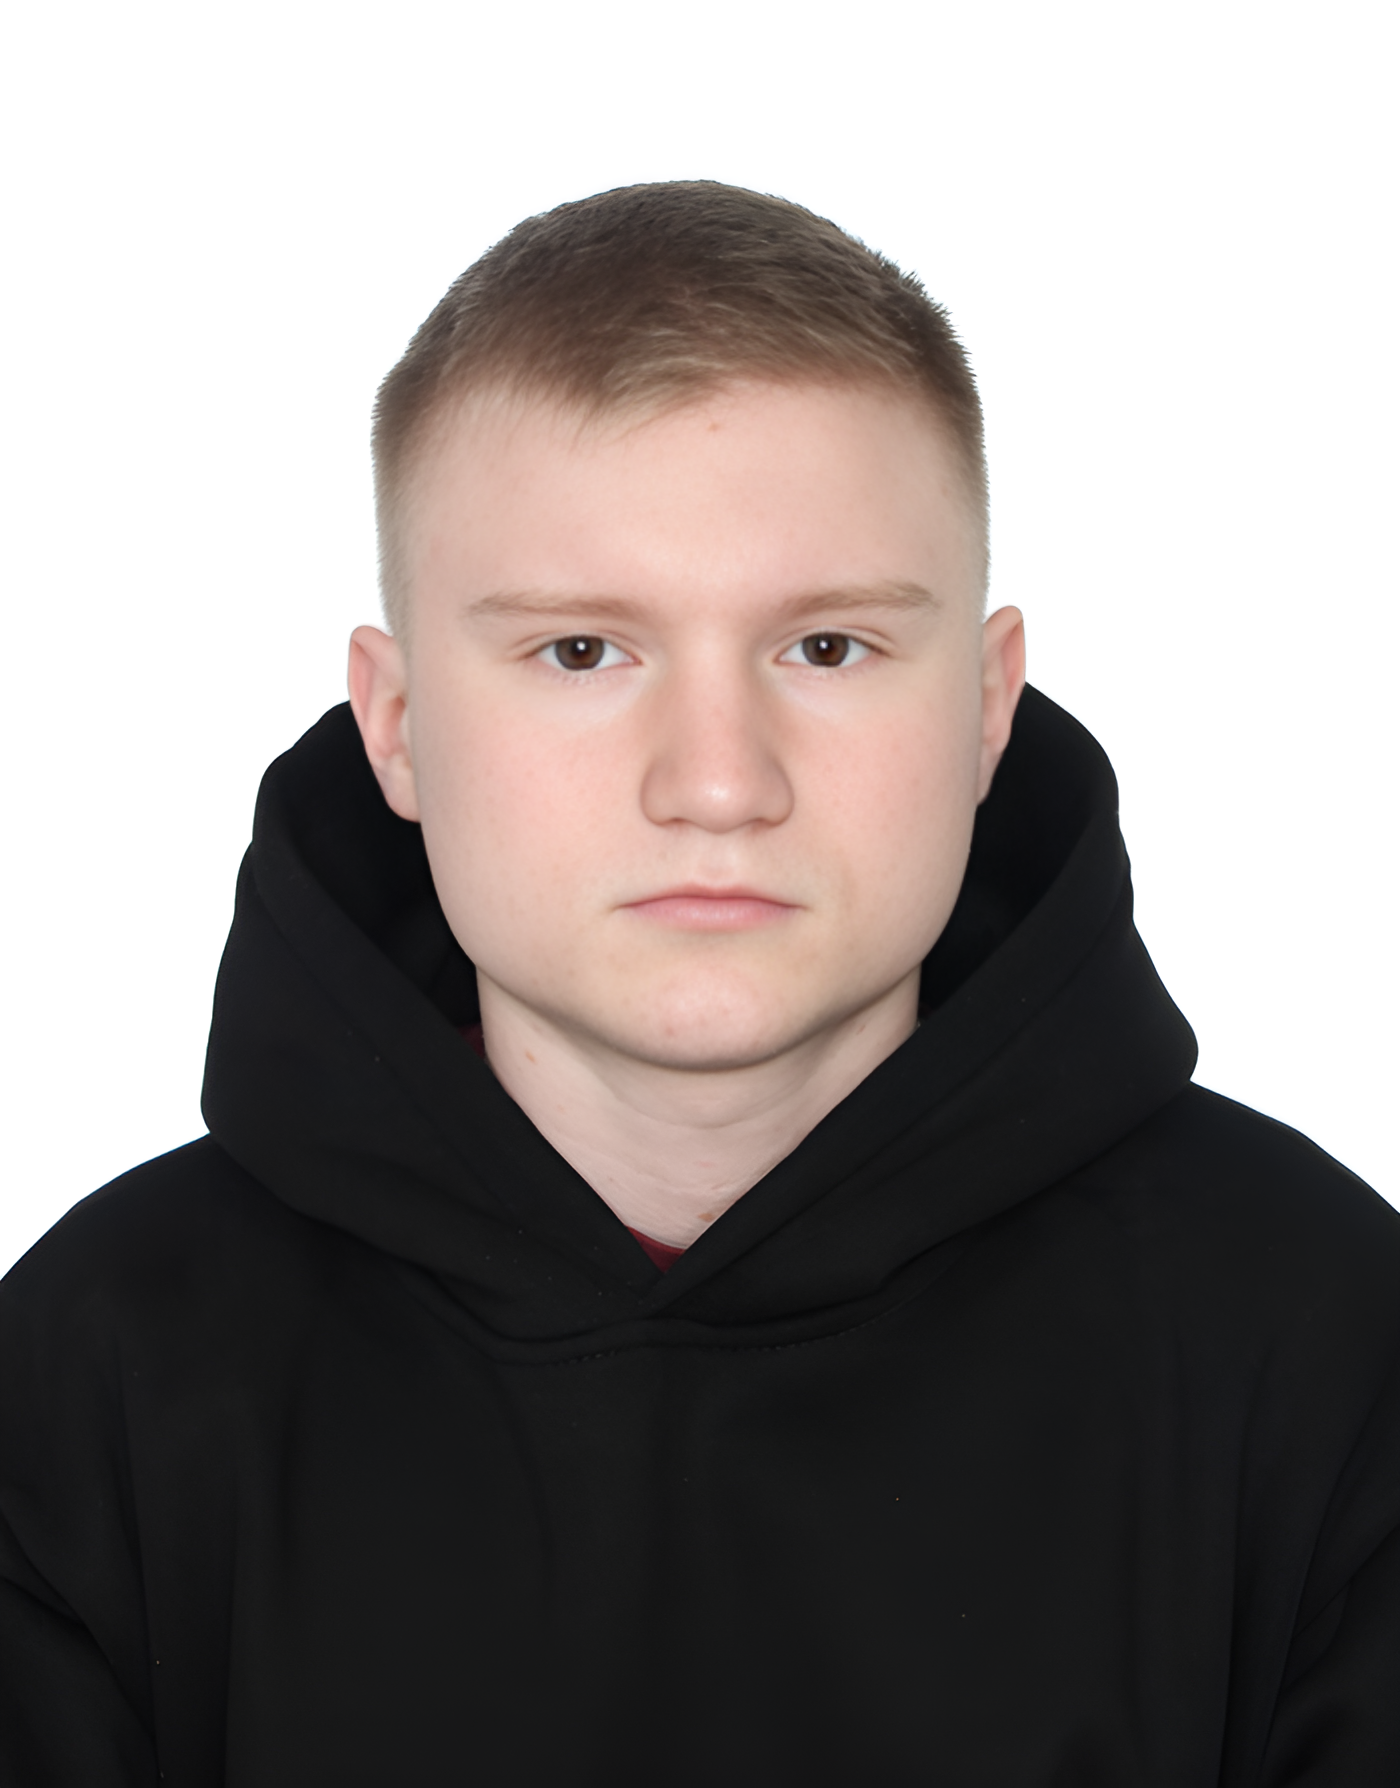
\includegraphics[width=2.8cm]{myphoto}}}


% Uncomment to add a third address
% \address{Address 3 line 1\\Address 3 line 2\\Address 3 line 3}
%-------------------------------------------------------------------------------

\begin{resume}

%-------------------------------------------------------------------------------
%	EDUCATION SECTION
%-------------------------------------------------------------------------------
\section{EDUCATION}
MIPT DREC, Bachelor of Applied Mathematics \& Physics. \\
Moscow, Russia\\
GPA: 7.82
%-------------------------------------------------------------------------------

%-------------------------------------------------------------------------------
%	PROJECTS SECTION
%-------------------------------------------------------------------------------
\section{PROJECTS}
\par
\textbf{\href{https://github.com/KirillLakhnov/Language}{C-like language}}: 
In this project I implemented semantic and lexical analysis of my own programming language using the recursive descent algorithm. I also made a language translator for a simplified assembler, which is processed in a virtual processor I wrote earlier. In my language you can use conditional operators, loops, variables, functions. Furthermore, I used graphwiz for debug and compiling a tree.

\par
\textbf{\href{https://github.com/KirillLakhnov/Mandelbrot}{Mandelbrot Set}}:
In this project I researched SIMD optimizations for construction the Maldenbrot's set. The results of my research you can see on my \href{https://github.com/KirillLakhnov/Mandelbrot}{GitHub}.

\par
\textbf{\href{https://github.com/KirillLakhnov/Alpha-blending}{Alpha-blending}}: 
Alpha-blending is the task of superimposing one picture on another. Here I continued researching SFML and SSE instructions. The results of my research you can see on my \href{https://github.com/KirillLakhnov/Alpha-blending}{GitHub}.

\par
\textbf{\href{https://github.com/KirillLakhnov/ASM_PRINTF}{Printf}}: 
In this project I implemented a simplified analog of the "printf" function on NASM, which supports specifiers such as: \%\%, \%b, \%d, \%c, \%o, \%s, \%x.


%-------------------------------------------------------------------------------

%-------------------------------------------------------------------------------
%	COMPUTER SKILLS SECTION
%-------------------------------------------------------------------------------
\section{COMPUTER\\SKILLS}

\textbf{Languages}: C/C++, x86-64 Assembly, \LaTeX, Python.
\\
\textbf{Tools}: Make, CMake, VSCode, git, graphwiz, SFML, QT.
\\
\textbf{Foreign language}: English(B1).
%-------------------------------------------------------------------------------

%-------------------------------------------------------------------------------
%	EXPERIENCE SECTION
%-------------------------------------------------------------------------------
% Modify the format of each position
\begin{format}
\title{l}\employer{r}\\
\dates{l}\location{r}\\
\body\\
\end{format}
%-------------------------------------------------------------------------------
%	Interests
%-------------------------------------------------------------------------------
\section{INTERESTS}
compilers, low-level optimization, operation systems, computer architecture, mathematics.
%-------------------------------------------------------------------------------
%-------------------------------------------------------------------------------
%	Achievements
%-------------------------------------------------------------------------------
\section{ACHIEVEMENTS}
Completed Huawei's course "C-Programming" in MIPT \\
Passed 6 out of 8 tasks from Huawei's Assembly and Architecture course \\
All-Russian Olympiad for Schoolchildren in Economics --- Two-time awardee of regional stage \\
All-Russian Olympiad for Schoolchildren in Economics --- Participant of the final stage \\
All-Russian Olympiad for Schoolchildren in Mathematics --- One-time awardee of regional stage \\
%-------------------------------------------------------------------------------
\end{resume}
\end{document}